

\chapter{\kernelTitle}\label{kernelrank}

Given a linear transformation \[L \colon V \to W\, ,\] we often want  to know if it has an inverse, {\itshape i.e.}, if there exists a linear transformation \[M \colon W \to V\] such that for any vector \(v \in V\), we have \[MLv=v\, ,\] and for any vector \(w \in W\), we have \[LMw=w\, .\] A linear transformation is a special kind of function from one vector space to another. So before we discuss which linear transformations have inverses, let us first discuss inverses of arbitrary functions. When we later specialize to linear transformations, we'll also find some nice ways of creating subspaces.

Let \(f \colon S \to T\) be a function from a set \(S\) to a set \(T\). \href{\webworkurl Homework0-Background/3/}{Recall} that \(S\) is called the {\itshape domain} of \(f\), \(T\) is called the {\itshape codomain} or {\itshape target} of \(f\).  
We now formally introduce a term that should be familar to you from many previous courses.

\section{Range}

\begin{definition} 
The {\bfseries range}  of a function $f:S\to T$ is  the set
\[
\range (f):=\left\{ f(s) | s\in S \right\}\subset T\, .
\]
%is called\(f\). 
\end{definition} 
It is the subset of the codomain consisting of elements  to which the function \(f\) maps, {\itshape i.e.}, the things in \(T\) which you can get to by starting in \(S\) and applying \(f\). 

The range of a matrix is very easy to find; the range of a matrix is the span of its columns. 
Thus, calculation of the range of a matrix is very easy until the last step: simplification. One aught to end by the calculation by writing the vector space as the span of a linearly independent set. 

\begin{example}{ of calculating the range of a matrix.}
\begin{gather*}\range  
\begin{pmatrix} 
1&2&0&1\\
1&2&1&2\\
0&0&1&1
\end{pmatrix} 
:= 
\left\{ 
\begin{pmatrix} 
1&2&0&1\\
1&2&1&2\\
0&0&1&1
\end{pmatrix} 
\colvec{x\\y\\z\\w } | \colvec{x\\y\\z\\w} \in \R^4 \right\}
\\=
\left\{   
x\colvec{1\\1\\0 } +y \colvec{ 2\\2\\0 } +z \colvec{0\\1\\1} + w\colvec{1\\2\\1} \middle| x,y,z,w \in \R \right\}
.\end{gather*}
That is 
\[
\range  
\begin{pmatrix} 
1&2&0&1\\
1&2&1&2\\
0&0&1&1
\end{pmatrix} 
= 
\spa \left\{   
\colvec{1\\1\\0 } , \colvec{ 2\\2\\0 } , \colvec{0\\1\\1}, \colvec{1\\2\\1} \right\}
\]
but since 
\[\rref\begin{pmatrix} 
1&2&0&1\\
1&2&1&2\\
0&0&1&1
\end{pmatrix} 
=\begin{pmatrix} 
1&2&0&1\\
0&0&1&1\\
0&0&0&0
\end{pmatrix} 
\]
the second and fourth columns (which are the non-pivot columns), can be expressed as linear combinations of columns to their left. 
They can then be removed from the set in the span to obtain
\[\range  
\begin{pmatrix} 
1&2&0&1\\
1&2&1&2\\
0&0&1&1
\end{pmatrix} 
= \spa \left\{   
\colvec{1\\1\\0 } , \colvec{0\\1\\1} \right\} .
\]
\end{example}

It might occur to you that the range of the $3\times 4$ matrix from the last example can be expressed as the range of a $3\times 2$ matrix;
\[
\range  
\begin{pmatrix} 
1&2&0&1\\
1&2&1&2\\
0&0&1&1
\end{pmatrix} 
=\range  
\begin{pmatrix} 
1&0\\
1&1\\
0&1
\end{pmatrix}.\]
Indeed, because the span of a set of vectors does not change when we replace the vectors with another set through an invertible process, we can calculate ranges through strings of equalities of ranges of matrices that differer by Elementary Column Operations, ECOs, ending with the range of a matrix in Column Reduced Echelon Form, CREF, with its zero columns deleted.

\begin{example} Calculating a range with ECOs\\
\begin{gather*}
\range  
\begin{pmatrix} 
0&1&1\\
1&3&1\\
1&2&0
\end{pmatrix} 
\stackrel{c_1 \leftrightarrow c_3}{=}
\range  
\begin{pmatrix} 
1&1&0\\
1&3&1\\
0&2&1
\end{pmatrix} 
\stackrel{c_2'= c_2-c_1}{=}
\range  
\begin{pmatrix} 
1&0&0\\
1&2&1\\
0&2&1
\end{pmatrix} 
\stackrel{c_2'= \frac12 c_2}{=}
\range  
\begin{pmatrix} 
1&0&0\\
1&1&1\\
0&1&1
\end{pmatrix} 
\\\stackrel{c_3'= c_3-c_2}{=}
\range  
\begin{pmatrix} 
1&0&0\\
1&1&0\\
0&1&0
\end{pmatrix} 
=\range  
\begin{pmatrix} 
1&0\\
1&1\\
0&1
\end{pmatrix}. 
\end{gather*}


\end{example}

\noindent
This is an efficient way to compute and encode the range of a matrix.
%We think this is the most sophisticated and efficient way to calculate the range of a matrix, and encourage students to use this line of thinking.

\section{Image} 

\begin{definition}
For any subset $U$ of the domain $S$ of a function $f:S\to T$  the {\bfseries image} of $U$ is 
\[f(U)=\Image U:= \left\{  f(x) | x\in U \right\} .\]
\end{definition}

\begin{example} 
The image of the  cube
\[U= \left\{  a \colvec{1\\0\\0} +b \colvec{0\\1\\0}+c\colvec{0\\0\\1} \middle| a,b,c \in [0,1] \right\} \] 
under multiplication by the matrix 
\[ M=
\begin{pmatrix}
1&0&0\\
1&1&1\\
0&0&1
\end{pmatrix}
\]
is the parallelepiped 
\[
\Img U= 
 \left\{  a \colvec{1\\1\\0} +b \colvec{0\\1\\0}+c\colvec{0\\1\\1} \middle| a,b,c \in [0,1] \right\} .
\]
\end{example}

Note that for most subsets $U$ of the domain $S$  of a function  $f$ the image of $U$ is not a vector space. 
The range of a function is the particular case of the image where the subset of the domain is the entire domain; $\range  f = \Img S$. 
For this reason, the range of $f$ is also sometimes called the \emph{image} of $f$ and is sometimes denoted $\im(f)$ or  $f(S).$  We have seen that the range of a matrix is always a span of vectors, and hence a vector space. 

Note that we prefer the phrase ``range of $f$" to the phrase ``image of f"  
because we wish to avoid confusion between homophones;
 the word 
``image" is also used to describe a single element of the codomain assigned to a single element of the domain. 
For example, 
one might say of 
the function $A:\mathbb{R}\to\mathbb{R}$ with rule of correspondence $A(x=)=2x-1$ for all $x$ in $\mathbb{R}$ that the image of $2$ is $3$ with this second meaning of the word ``image" in mind. 
By contrast, one would never say that the range of $2$ is $3$ since the former is not a function and the latter is not a set.


For thinking about inverses of function we want to think in the oposite direction in a sense. 
\begin{definition} 
The {\bfseries pre-image}\index{Pre-image} of any subset $U \subset T$ is 
\[
f^{-1}(U):=\{ s\in S | f(s)\in U \}\subset S.
\]
\end{definition}
The pre-image of a set \(U\) is the set of all elements of \(S\) which map to \(U\). 
\begin{example}
The pre-image of the set $U= \left\{ a\colvec{2\\1\\1 } \middle| a\in [0,1]\right\}$ (a line segment) under the matrix 
\[ 
M=\begin{pmatrix}
1&0&1\\
0&1&1\\
0&1&1
\end{pmatrix}: \R^3\to \R^3
\]
is the set 
\begin{align*}
M^{-1} U&= \left\{  x \middle| Mx=v \text{~for~some~} v\in U \right\} \\[3mm]
&= \left\{  \colvec{x\\y\\z} \middle| 
\begin{pmatrix}
1&0&1\\
0&1&1\\
0&1&1
\end{pmatrix} \colvec{x\\y\\z} =a\colvec{2\\1\\1}  \text{~for~some~} a\in [0,1] \right\} .
\end{align*}
Since
\[
\rref
\begin{amatrix}{3}
1&0&1&2a\\
0&1&1&a\\
0&1&1&a
\end{amatrix} 
= 
\begin{amatrix}{3}
1&0&1&2a\\
0&1&1&a\\
0&0&0&0
\end{amatrix} 
\]
we have 
\[ M^{-1} U = \left\{   a \colvec{2\\1\\0} +b \colvec{-1\\-1\\ 1}\,  \middle|\,  a\in [0,1] ,b\in \R\right\},\]
a strip from a plane in $\R^3$.
\end{example}


\begin{figure}
\begin{center}
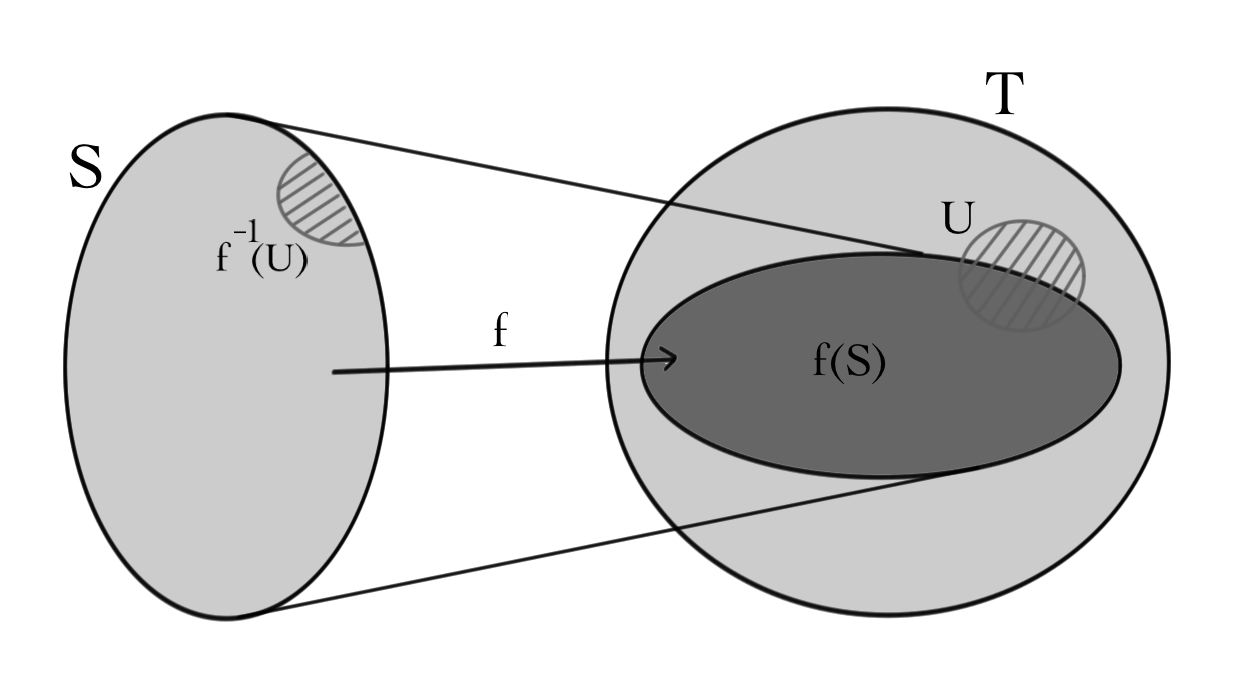
\includegraphics[scale=.25]{functions.jpg}
\end{center}
\caption{For the function $f:S\to T$, $S$ is the domain\index{Domain}, $T$ is the target/codomain\index{Codomain}\index{Target|see{Codomain}}, $f(S)$ is the range and $f^{-1}(U)$ is the
pre-image of $U\subset T$.}
\end{figure}

\subsection{ One-to-one and Onto}
The function \(f\) is {\bfseries one-to-one} (sometimes denoted 1:1) if different elements in \(S\) always map to different elements in \(T\). That is, \(f\) is one-to-one if for any elements \(x \neq y \in S,\) we have that \(f(x) \neq f(y)\), as pictured below.
\begin{center}
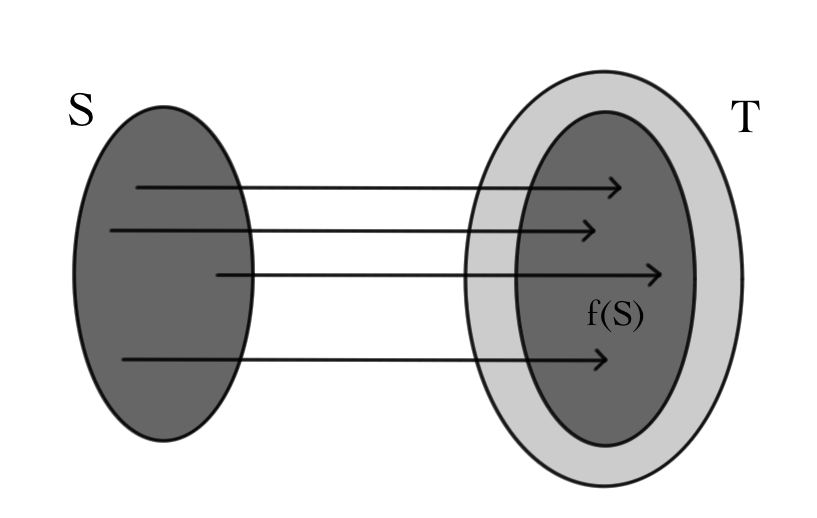
\includegraphics[scale=.25]{121.jpg}
\end{center} 
One-to-one functions are also called {\bfseries injective} functions (and sometimes called monomorphisms.) Notice that injectivity is a condition on the pre-images of \(f\).

The function \(f\) is {\bfseries onto} if every element of \(T\) is mapped to by some element of \(S\). That is, \(f\) is onto if for any \(t \in T\), there exists some \(s \in S\) such that \(f(s)=t\). Onto functions are also called {\bfseries surjective} functions (and sometimes epimorphisms.) Notice that surjectivity is a condition on the range of \(f\).
\begin{center}
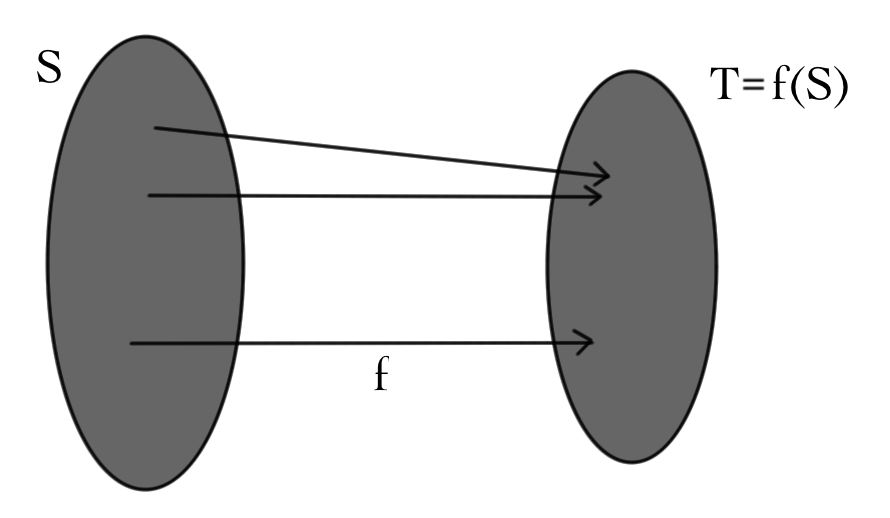
\includegraphics[scale=.25]{onto.jpg}
\end{center} 

If \(f\) is both injective and surjective, it is {\bfseries bijective} (or an isomorphism.)
\begin{center}
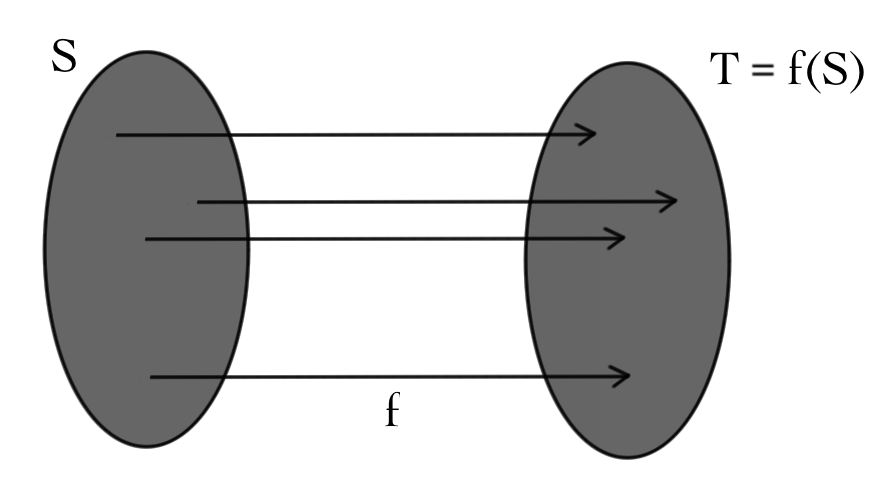
\includegraphics[scale=.25]{biject.jpg}
\end{center} 
\begin{theorem}
A function \(f \colon S \to T\) has an inverse function \(g \colon T \to S\) if and only if $f$ is bijective.
\end{theorem}
\begin{proof}
This is an ``if and only if'' statement  so the proof has two parts.
\begin{enumerate}
\item {\itshape (Existence of an inverse $\Rightarrow$ bijective.)}

Suppose that \(f\) has an inverse function \(g\). We need to show $f$ is bijective, which
we break down into injective and surjective.
\begin{itemize}
\item The function \(f\) is injective: 
Suppose that we have \(s,s' \in S\) such that \(f(s)=f(s')\). We must have that \(g(f(s))=s\) for any \(s \in S\), so in particular \(g(f(s))=s\) and \(g(f(s'))=s'\). But since \(f(s)=f(s'),\) we have \(g(f(s))=g(f(s'))\) so \(s=s'\). Therefore, \(f\) is injective.

\item The function \(f\) is surjective:
Let \(t\) be any element of \(T\). We must have that \(f(g(t))=t\). Thus, \(g(t)\) is an element of \(S\) which maps to \(t\). So \(f\) is surjective.
\end{itemize}

\item {\itshape (Bijectivity $\Rightarrow$ existence of an inverse.)}
Suppose that \(f\) is bijective. Hence \(f\) is surjective, so every element \(t \in T\) has at least one pre-image. Being bijective, \(f\) is also injective, so every \(t\) has no more than one pre-image. Therefore, to construct an inverse function \(g\), we simply define \(g(t)\) to be the unique pre-image \(f^{-1}(t)\) of \(t\).
\end{enumerate}
\end{proof}

Now let us specialize to functions \(f\) that are linear maps between two vector spaces. Everything we said above for arbitrary functions is exactly the same for linear functions. However, the structure of vector spaces lets us say much more about one-to-one and onto functions whose domains are vector spaces than we can say about functions on general sets.  For example, we know that a linear function always sends $0_V$ to $0_W$, {\itshape i.e.},
\Shabox{1.1}{$f(0_V)=0_W$}  
In Review Exercise~\ref{injectivekernalprob}, you will show that a linear transformation is one-to-one if and only if $0_V$ is the only vector that is sent to $0_W$. Linear functions are unlike  arbitrary functions between sets in that, by looking at {\itshape just one} (very special) vector, we can figure out whether $f$ is one-to-one!  
\subsection{Kernel}
Let \(L \colon V \to W\) be a linear transformation. Suppose \(L\) is \emph{not} injective.  Then we can find $v_1 \neq v_2$ such that $Lv_1=Lv_2$.  So $v_1-v_2\neq 0$, but
\[
L(v_1-v_2)=0.
\]

\begin{definition}
If $L \colon V\rightarrow W$ is a linear function  then the set 
\index{Kernel}
\[
\ker L = \{v\in V ~|~ Lv=0_W \}\subset V 
\]
is called the {\bfseries kernel of $L$}.
\end{definition}


Notice that if $L$ has matrix $M$ in some basis, then finding the kernel of~$L$ is equivalent to solving the homogeneous system 
\[
MX=0.
\]

\begin{example}
Let $L(x,y)=(x+y,x+2y,y)$.  Is $L$ one-to-one?

To find out, we can solve the linear system:
\[
\begin{amatrix}{2}
1 & 1 & 0 \\
1 & 2 & 0 \\
0 & 1 & 0 \\
\end{amatrix} \sim
\begin{amatrix}{2}
1 & 0 & 0 \\
0 & 1 & 0 \\
0 & 0 & 0 \\
\end{amatrix}.
\]
Then all solutions of $MX=0$ are of the form $x=y=0$.  In other words, $\ker L=\{0\}$, and so $L$ is injective.
\end{example}

%\begin{center}\href{\webworkurl ReadingHomework24/1/}{Reading homework: problem \ref{kernelrank}.1}\end{center}
\Reading{KernelRangeNullityRank}{1}

Notice that in the above example we found 
\[\ker 
\begin{pmatrix}
1 & 1  \\
1 & 2  \\
0 & 1 \\
\end{pmatrix} =
\ker
\begin{pmatrix}
1 & 0 \\
0 & 1  \\
0 & 0  \\
\end{pmatrix}.
\]
In general, an efficient way to get the  kernel of a matrix is to write a string of equalities between kernels of matrices which differ by row operations and, once RREF is reached, note that the linear relationships between the columns for a basis for the nullspace.

\begin{example} of calculating the kernel of a matrix.\\
\begin{gather*}
\ker 
\begin{pmatrix}
1&2&0&1 \\
1&2&1&2 \\
0&0&1&1
\end{pmatrix}
=
\ker 
\begin{pmatrix}
1&2&0&1 \\
0&0&1&1 \\
0&0&1&1
\end{pmatrix}
=
\ker 
\begin{pmatrix}
1&2&0&1 \\
0&0&1&1 \\
0&0&0&0
\end{pmatrix}
\\
=\spa \left\{ 
\colvec{-2\\1 \\0\\0}, \colvec{-1\\0\\-1 \\1 } 
 \right\} .
\end{gather*}
The two column vectors in this last line describe linear relations between the columns $c_1,c_2,c_3,c_4$. 
In particular $-2c_1+1c_2=0$ and $-c_1-c_3 +c_4=0$. 
\end{example}
In general, a description of the kernel of a matrix should be of the form 
$\spa \{ v_1,v_2,\dots,v_n\}$ with one vector $v_i$ for each non-pivot column. 
To agree with the standard procedure, think about how to describe each non-pivot column in terms of columns to its left; this will yield an expression of the form wherein each vector  has a 1 as its last non-zero entry. (Think of Column Reduced Echelon Form, CREF.) 

Thinking again of augmented matrices, 
if a matrix has more than one element in its kernel then it is not invertible since the existence of multiple solutions to $Mx=0$ implies that $\rref M\neq I$. 
However just because the kernel of a linear function is trivial does not mean that the function is invertible. 

\begin{example}
$\ker 
\begin{pmatrix}
1&0\\
1&1\\
0&1
\end{pmatrix} =\left\{  \colvec{0\\0} \right\} $
since the matrix has no non-pivot columns. However, 
$\begin{pmatrix}
1&0\\
1&1\\
0&1
\end{pmatrix}:  \R^2 \to \R^3$
is not invertible because there are many things in its codomain that are not in its range, such as  $\colvec{1\\0\\0}$. 
\end{example}

A trivial kernel only gives us half of what is needed for invertibility.




\begin{theorem}
A linear transformation $L\colon V\rightarrow W$ is injective iff \[\ker L=\{0_V\}\, .\]
\end{theorem}

\begin{proof}
The proof of this theorem is Review Exercise~\ref{injectivekernalprob}.
\end{proof}



\begin{theorem}
If $L \colon V\stackrel{\textrm{linear}}{-\!\!\!-\!\!\!-\!\!\!\rightarrow} W$  then $\ker L$ is a subspace of $V$.
\end{theorem}

\begin{proof}
Notice that if $L(v)=0$ and $L(u)=0$, then for any constants $c,d$, $L(cu+dv)=0$.  Then by the \hyperref[subspacetheorem]{subspace theorem}, the kernel of $L$ is a subspace of $V$.
\end{proof}

\begin{example}
Let \(L \colon \Re^3 \to \Re\) be the linear transformation defined by \(L(x,y,z)=(x+y+z)\). Then \(\ker L\) consists of all vectors \((x,y,z) \in \Re^3\) such that \(x+y+z=0\). Therefore, the set
\[
V=\{(x,y,z) \in \Re^3 \mid x+y+z=0\}
\]
is a subspace of \(\Re^3\).
\end{example}

When $L:V\to V$, the above theorem has an interpretation in terms of the eigenspaces of $L$. Suppose $L$ has a zero eigenvalue.  Then the associated eigenspace consists of all vectors $v$ such that $Lv=0v=0$; the $0$-eigenspace of $L$ is exactly the kernel of $L$.  



In the example where $L(x,y)=(x+y,x+2y,y)$, the map $L$ is clearly not surjective, since $L$ maps $\Re^2$ to a plane through the origin in $\Re^3$. But any plane through the origin is a subspace. In general notice 
that if $w=L(v)$ and $w'=L(v')$, then for any constants $c,d$, linearity of $L$ ensures that \[cw+dw' = L(cv+dv')\, .\]  Now the subspace theorem strikes again, and we have the following theorem:

\begin{theorem}
If $L \colon V\rightarrow W$ is linear then the range $L(V)$ is a subspace of~$W$.
\end{theorem}

\begin{example}
Let $L(x,y)=(x+y,x+2y,y)$. The range of $L$ is a plane through the origin and thus a subspace of ${\mathbb R}^3$.
Indeed the matrix of $L$ in the standard basis is 
\[
\begin{pmatrix}1&1\\1&2\\0&1\end{pmatrix}\, .
\]
The columns of this matrix encode the possible outputs of the function $L$ because
\[
L(x,y)=\begin{pmatrix}1&1\\1&2\\0&1\end{pmatrix}\colvec{x\\ y}=x \colvec{1\\1\\0}+y\colvec{1\\2\\1}\, . 
\]
Thus 
\[
L({\mathbb R}^2)=\spa \left\{\colvec{1\\1\\0},\colvec{1\\2\\1}\right\}
\]
Hence, when  bases and a linear transformation is are given, people often refer to its range as the {\itshape column space}\index{Column space}
of the corresponding matrix.
\end{example}

To find a basis of the range of $L$, we can start with a basis $S=\{v_1, \ldots, v_n\} $ for $V$. Then
the most general input for $L$ is of the form  $\alpha^1 v_1 + \cdots + \alpha^n v_n$. In turn, its most general output looks like
\[
L\big(\alpha^1 v_1 + \cdots + \alpha^n v_n\big)=\alpha^1 Lv_1 + \cdots + \alpha^n Lv_n\in \spa\{Lv_1,\ldots\,Lv_n\}\, .
\]
Thus
\[
L(V)=\spa L(S) = \spa \{Lv_1, \ldots, Lv_n\}\, .
\]
However, the set $\{Lv_1, \ldots, Lv_n\}$ may not be linearly independent; we must solve 
\[
c^1Lv_1+ \cdots + c^nLv_n=0\, ,
\]
to determine whether it is.
By finding relations amongst the elements of $L(S)=\{Lv_1,\ldots ,L v_n\}$, we can discard vectors until a basis is arrived at.  The size of this basis is the dimension of the range of $L$, which is known as the \emph{rank}\index{Rank} of $L$.


\begin{definition}
The {\bfseries rank} of a linear transformation $L$ is the dimension of its range.
The {\bfseries nullity}\index{Nullity} of a linear transformation is the dimension of the kernel.
\end{definition}
The notation for these numbers is 
 \Shabox{1}{$\nul L:=\dim \ker L$,}  
 \Shabox{1}{$\rank L:=\dim L(V) = \dim\, \text{ran}\, L$.} 

\begin{theorem}[Dimension Formula]\index{Dimension formula}\label{dimension_formula}
Let $L \colon V\rightarrow W$ be a linear transformation, with $V$ a finite-dimensional vector space\footnote{The formula still makes sense for infinite dimensional vector spaces, such as the space of all polynomials, but the notion of a basis for an infinite dimensional space is more sticky than in the finite-dimensional case.  Furthermore, the dimension formula for infinite dimensional vector spaces isn't useful for computing the rank of a linear transformation, since an equation like $\infty=\infty+x$ cannot be solved for $x$. As such, the proof presented assumes a finite basis for $V$.}.  Then:
\begin{align*}
\dim V &= \dim \ker V + \dim L(V)\\
 &= \nul L + \rank L.
\end{align*}
\end{theorem}



\begin{proof}
Pick a basis for $V$:
\[
\{ v_1,\ldots,v_p,u_1,\ldots, u_q \},
\]
where $v_1,\ldots,v_p$ is also a basis for $\ker L$.  This can always be done, for example, by finding a basis for the kernel of $L$ and then extending to a basis for $V$.  Then $p=\nul L$ and $p+q=\dim V$.  Then we need to show that $q=\rank L$.  To accomplish this, we show that 
$\{L(u_1),\ldots,L(u_q)\}$ is a basis for $L(V)$.

To see that $\{L(u_1),\ldots,L(u_q)\}$ spans $L(V)$, consider any vector $w$ in $L(V)$.  Then we can find constants $c^i, d^j$ such that:
\begin{align*}
w &= L(c^1v_1 + \cdots + c^pv_p+d^1u_1 + \cdots + d^qu_q)\\
  &= c^1L(v_1) + \cdots + c^pL(v_p)+d^1L(u_1)+\cdots+d^qL(u_q)\\
  &= d^1L(u_1)+\cdots+d^qL(u_q) \text{ since $L(v_i)=0$,}\\
\Rightarrow L(V) &= \spa \{L(u_1), \ldots, L(u_q)  \}.
\end{align*}

Now we show that $\{L(u_1),\ldots,L(u_q)\}$ is linearly independent.  We argue by contradiction. Suppose there exist constants $d^j$ (not all zero) such that
\begin{align*}
0 &= d^1L(u_1)+\cdots+d^qL(u_q)\\
  &= L(d^1u_1+\cdots+d^qu_q).
\end{align*}
But since the $u^j$ are linearly independent, then $d^1u_1+\cdots+d^qu_q\neq 0$, and so $d^1u_1+\cdots+d^qu_q$ is in the kernel of $L$.  But then $d^1u_1+\cdots+d^qu_q$ must be in the span of $\{v_1,\ldots, v_p\}$, since this was a basis for the kernel.  This contradicts the assumption that $\{ v_1,\ldots,v_p,u_1,\ldots, u_q \}$ was a basis for $V$, so we are done.
\end{proof}

%\begin{center}\href{\webworkurl ReadingHomework24/2/}{Reading homework: problem \ref{kernelrank}.2}\end{center}
\Reading{KernelRangeNullityRank}{2}

\begin{example} (Row rank equals column rank)\\
Suppose $M$ is an $m\times n$ matrix. The matrix  $M$ itself is a linear transformation $M:{\mathbb R}^n \rightarrow {\mathbb R}^m$ but it  must also  be the matrix of some linear transformation
\[
L:V\stackrel{\textrm{linear}}\longrightarrow W\, .
\]
Here we only know that $\dim V =n$ and $\dim W =m$. The rank of the map $L$ is the dimension of its image and also the number of linearly independent columns of $M$. Hence, this is sometimes called the \index{Rank!column rank}{\itshape column rank} of $M$. The dimension formula predicts  the dimension of the kernel, {\itshape i.e.} the nullity:  $ \null L= \dim V-\rank L=n-r$. 

To compute the kernel we would study the linear system \[Mx=0\, ,\] which gives $m$ equations for the $n$-vector~$x$. The \index{Rank!row rank}{\itshape row rank} of a matrix is the number of linearly independent rows (viewed as vectors).
Each linearly independent row of $M$ gives an independent equation satisfied by the $n$-vector $x$. Every independent equation on $x$ reduces the size of the kernel by one, so if the row rank is $s$, then $\null L+ s = n$.  Thus we have two equations: 
\[
\null L+s=n \text{ and } \null L = n-r\, .
\]
From these we conclude the $r=s$. In other words, the row rank of $M$ equals its column rank.
 \end{example}



\section{Summary}\label{thelist}
We have seen that a linear transformation has an inverse if and only if it is bijective ({\itshape i.e.}, one-to-one and onto). We also know that linear transformations can be represented by matrices, and we have seen many ways to tell whether a matrix is invertible. Here is a list of them:
\begin{theorem}[Invertibility]
\label{theorem:invertibility}
Let $V$  be an $n$-dimensional vector space  
and suppose  $L:V\to V$ is a linear transformation with matrix $M$ in some basis.
Then \(M\) is an \(n \times n\) matrix, and 
%let \[L \colon \Re^n \to \Re^n\] be the linear transformation defined by \(L(v)=Mv\). Then 
the following statements are equivalent:
\newpage
\begin{enumerate}
\item If $v$ is any vector in \(\Re^n\), then the system \(Mx=v\) has exactly one solution.
\item The matrix \(M\) is row-equivalent to the identity matrix.
\item If \(v\) is any vector in \(V\), then \(L(x)=v\) has exactly one solution.
\item The matrix \(M\) is invertible.
\item The homogeneous system \(Mx=0\) has no non-zero solutions.
\item The determinant of \(M\) is not equal to \(0\).
%\item The matrix \(M\) is a product of elementary matrices of the form \(E_j^i, R^i(\lambda), S_j^i(\gamma)\) with \(\lambda \neq 0\).
\item The transpose matrix \(M^T\) is invertible.
\item The matrix \(M\) does not have \(0\) as an eigenvalue.
\item The linear transformation \(L\) does not have \(0\) as an eigenvalue.
\item The characteristic polynomial \(\det(\lambda I-M)\) does not have \(0\) as a root.
\item The columns (or rows) of \(M\) span \(\Re^n\).
\item The columns (or rows) of \(M\) are linearly independent.
\item The columns (or rows) of \(M\) are a basis for \(\Re^n\).
\item The linear transformation \(L\) is injective.
\item The linear transformation \(L\) is surjective.
\item The linear transformation \(L\) is bijective.
\end{enumerate}
\end{theorem}
Note: it is important that \(M\) be an \(n \times n\) matrix! If \(M\) is not square, then it can't be invertible, and many of the statements above are no longer equivalent to each other.
%I hate it when books do this. "Here is our proof: you prove it or figure out where it has been proven. " I think it is dishonest to write proof: and then not actually give a proof.
%Yes, but some books make proving the above list there raison d'être which I really don't like...plus we have a video handling this!!!!
\begin{proof}
Many of these equivalences were proved earlier in other chapters. Some were left as review questions or sample final questions. The rest are left as exercises for the reader.
\end{proof}

\Videoscriptlink{kernel_range_nullity_rank_inv_cond.mp4}{Invertibility Conditions}{scripts_kernel_range_nullity_rank_inv_cond}

%\section*{References}
%Hefferon, Chapter Three, Section II.2: Rangespace and Nullspace (Recall that ``homomorphism'' is is used instead of ``linear transformation'' in Hefferon.)
%\\
%Beezer, Chapter LT, Sections ILT-IVLT
%\\
%Wikipedia:
%\begin{itemize}
%\item \href{http://en.wikipedia.org/wiki/Rank_(linear_algebra)}{Rank}
%\item \href{http://en.wikipedia.org/wiki/Dimension_theorem}{Dimension Theorem}
%\item \href{http://en.wikipedia.org/wiki/Kernel_(linear_operator)}{Kernel of a Linear Operator}
%\end{itemize}

\section{Review Problems}

{\bfseries Webwork:} 
\begin{tabular}{|c|c|}
\hline
Reading Problems & 
 \hwrref{KernelRangeRankNullity}{1}, 
 \hwrref{KernelRangeRankNullity}{2}, 
 \\
Elements of kernel &  \hwref{KernelRangeRankNullity}{3}\\
Basis for column space &\hwref{KernelRangeRankNullity}{4}\\
Basis for kernel & \hwref{KernelRangeRankNullity}{5}\\
Basis for kernel and range& \hwref{KernelRangeRankNullity}{6}\\
Orthonomal range basis&\hwref{KernelRangeRankNullity}{7}\\
Orthonomal kernel basis&\hwref{KernelRangeRankNullity}{8}\\
Orthonomal kernel and range bases&\hwref{KernelRangeRankNullity}{9}\\
Orthonomal kernel,  range and row space bases&\hwref{KernelRangeRankNullity}{10}\\
Rank&\hwref{KernelRangeRankNullity}{11}\\
   \hline
\end{tabular}






\begin{enumerate}
\item \label{det33} Let $M=\begin{pmatrix}
m^1_1 & m^1_2 & m^1_3\\
m^2_1 & m^2_2 & m^2_3\\
m^3_1 & m^3_2 & m^3_3\\
\end{pmatrix}$.  Use row operations to put $M$ into \emph{row echelon form}.  For simplicity, assume that $m_1^1\neq 0 \neq m^1_1m^2_2-m^2_1m^1_2$.

Prove that $M$ is non-singular if and only if:
\[
m^1_1m^2_2m^3_3 
- m^1_1m^2_3m^3_2 
+ m^1_2m^2_3m^3_1 
- m^1_2m^2_1m^3_3 
+ m^1_3m^2_1m^3_2
- m^1_3m^2_2m^3_1
\neq 0
\]

\phantomnewpage

\item 
\begin{enumerate}
\item What does the matrix $E^1_2=\begin{pmatrix}
0 & 1 \\
1 & 0
\end{pmatrix}$ do to $M=\begin{pmatrix}
a & b \\
d & c
\end{pmatrix}$ under left multiplication?  What about right multiplication?
\item Find elementary matrices $R^1(\lambda)$ and $R^2(\lambda)$ that respectively multiply rows $1$ and $2$ of $M$ by $\lambda$ but otherwise leave $M$ the same under left multiplication.
\item Find a matrix $S^1_2(\lambda)$ that adds a multiple $\lambda$ of row $2$ to row $1$ under left multiplication.
\end{enumerate}

\phantomnewpage

\item Let $M$ be a matrix and $S^i_jM$ the same matrix with rows \(i\) and \(j\) switched.  Explain every line of the 
\hyperlink{rowswap}{series of equations} proving that $\det M = -\det (S^i_jM)$.

\phantomnewpage

%\item \label{prob_inversion_number} This problem is a ``hands-on'' look at why \hyperlink{permutation_parity}{the property} describing the parity of permutations is true.
%
%\hypertarget{inversion_number}{The \emph{inversion number}}\index{Permutation!Inversion number} of a permutation $\sigma$ is the number of pairs $i<j$ such that $\sigma(i)>\sigma(j)$; it's the number of ``numbers that appear left of smaller numbers'' in the permutation.  For example, for the permutation $\rho = [4,2,3,1]$, the inversion number is $5$. The number $4$ comes before $2,3,$ and $1$, and $2$ and $3$ both come before $1$.
%
%Given a permutation $\sigma$, we can make a new permutation $\tau_{i,j} \sigma$ by exchanging the $i$th and $j$th entries of $\sigma$.
%
%\begin{enumerate}
%\item What is the inversion number of the permutation \(\mu=[1,2,4,3]\) that exchanges 4 and 3 and leaves everything else alone? Is it an even or an odd permutation?
%
%\item What is the inversion number of the permutation \(\rho=[4,2,3,1]\) that exchanges 1 and 4 and leaves everything else alone? Is it an even or an odd permutation?
%
%\item What is the inversion number of the permutation \(\tau_{1,3} \mu\)? Compare the parity\footnote{The \emph{parity} of an integer refers to whether the integer is even or odd. Here the parity of a permutation $\mu$ refers to the parity of its inversion number.} of \(\mu\) to the parity of \(\tau_{1,3} \mu.\)
%
%\item What is the inversion number of the permutation \(\tau_{2,4} \rho\)? Compare the parity of \(\rho\) to the parity of \(\tau_{2,4} \rho.\)
%
%\item What is the inversion number of the permutation \(\tau_{3,4} \rho\)? Compare the parity of \(\rho\) to the parity of \(\tau_{3,4} \rho.\)
%\end{enumerate}
%
%\videoscriptlink{elementary_matrices_determinant_hint.mp4}{Problem~\ref{prob_inversion_number} hints}{scripts_elementary_matrices_determinants_hint}

\phantomnewpage

%\item \label{problem_permutation} (Extra credit) Here we will examine a (very) small set of the general properties about permutations and their applications. In particular, we will show that one way to compute the sign of a permutation is by finding the \hyperlink{inversion_number}{inversion number} $N$ of $\sigma$ and we have
%\[
%\sgn(\sigma) = (-1)^N.
%\]
%
%For this problem, let $\mu = [1,2,4,3]$.
%
%\begin{enumerate}
%\item Show that every permutation $\sigma$ can be sorted by only taking simple (adjacent) transpositions\index{Permutation!Simple transposition} $s_i$ where $s_i$ interchanges the numbers in position $i$ and $i+1$ of a permutation $\sigma$ (in our other notation $s_i = \tau_{i,i+1}$). For example $s_2 \mu = [1, 4, 2, 3]$, and to sort $\mu$ we have $s_3 \mu = [1, 2, 3, 4]$.
%
%\item \label{prob_part_relations} We can compose simple transpositions together to represent a permutation (note that the sequence of compositions is not unique), and these are associative, we have an identity (the trivial permutation where the list is in order or we do nothing on our list), and we have an inverse since it is clear that $s_i s_i \sigma = \sigma$. Thus permutations of $[n]$ under composition are an example of a \hyperref[groups]{group}. However note that not all simple transpositions commute with each other since
%\begin{align*}
%s_1 s_2 [1, 2, 3] & = s_1 [1, 3, 2] = [3, 1, 2]
%\\ s_2 s_1 [1, 2, 3] & = s_2 [2, 1, 3] = [2, 3, 1]
%\end{align*}
%(you will prove here when simple transpositions commute). When we consider our initial permutation to be the trivial permutation $e = [1, 2, \dotsc, n]$, we do not write it; for example $s_i \equiv s_i e$ and $\mu = s_3 \equiv s_3 e$. This is analogous to not writing 1 when multiplying. Show that $s_i s_i = e$ (in shorthand $s_i^2 = e$), $s_{i+1} s_i s_{i+1} = s_i s_{i+1} s_i$ for all $i$, and $s_i$ and $s_j$ commute for all $|i - j| \geq 2$.
%
%\item Show that every way of expressing $\sigma$ can be obtained from using the relations proved in part~\ref{prob_part_relations}. In other words, show that for any expression $w$ of simple transpositions representing the trivial permutation $e$, using the proved relations.
%
%\emph{Hint: Use induction on $n$. For the induction step, follow the path of the $(n+1)$-th strand by looking at $s_n s_{n-1} \cdots s_k s_{k\pm1} \cdots s_n$ and argue why you can write this as a subexpression for any expression of $e$. Consider using diagrams of these paths to help.}
%
%\item The simple transpositions \hyperlink{action}{acts on} an $n$-dimensional vector space $V$ by $s_i v = E^i_{i+1} v$ (where $E^i_j$ is \hyperlink{elem_matrix_row_swap}{an elementary matrix}) for all vectors $v \in V$. Therefore we can just represent a permutation $\sigma$ as the matrix $M_{\sigma}$\footnote{Often people will just use $\sigma$ for the matrix when the context is clear.}, and we have $\det(M_{s_i}) = \det(E^i_{i+1}) = -1$. Thus prove that $\det(M_{\sigma}) = (-1)^N$ where $N$ is a number of simple transpositions needed to represent $\sigma$ as a permutation. You can assume that $M_{s_i s_j} = M_{s_i} M_{s_j}$ (it is not hard to prove) and that $\det(A B) = \det(A) \det(B)$ \hyperref[detmultiplicative]{from Chapter~\ref*{elementarydeterminantsII}}.
%
%\emph{Hint: You to make sure $\det(M_{\sigma})$ is well-defined since there are infinite ways to represent $\sigma$ as simple transpositions.}
%
%\item Show that $s_{i+1} s_i s_{i+1} = \tau_{i, i+2}$, and so give one way of writing $\tau_{i, j}$ in terms of simple transpositions? Is $\tau_{i,j}$ an even or an odd permutation? What is $\det(M_{\tau_{i,j}})$? What is the inversion number of $\tau_{i,j}$?
%
%\item The minimal number of simple transpositions needed to express $\sigma$ is called the \emph{length}\index{Permutation!Length} of $\sigma$; for example the length of $\mu$ is 1 since $\mu = s_3$. Show that the length of $\sigma$ is equal to the inversion number of $\sigma$.
%
%\emph{Hint: Find an procedure which gives you a new permutation $\sigma^{\prime}$ where $\sigma = s_i \sigma^{\prime}$ for some $i$ and the inversion number for $\sigma^{\prime}$ is 1 less than the inversion number for $\sigma$.}
%
%\item Show that $(-1)^N = \sgn(\sigma) = \det(M_{\sigma})$, where $\sigma$ is a permutation with $N$ inversions. Note that this immediately implies that $\sgn(\sigma \rho) = \sgn(\sigma) \sgn(\rho)$ for any permutations $\sigma$ and $\rho$.
%\end{enumerate}

\item Let $M'$ be the matrix obtained from $M$ by swapping two columns $i$ and $j$. Show that $\det M'=-\det M $.

\item The scalar triple product of three vectors $u,v,w$ from $\Re^3$ is $u\cdot(v\times w)$. Show that this product is the same as the determinant of the matrix whose columns are $u,v,w$ (in that order). What happens to the scalar triple product when the factors are permuted? 

\item Show that if $M$ is a $3\times 3$ matrix whose third row is a sum of multiples of the other rows ($R_3=aR_2+bR_1$) then $\det M=0$. Show that the same is true if one of the columns is a sum of multiples of the others. 

\end{enumerate}

\phantomnewpage

\newpage
